\documentclass[aspectratio=43]{beamer}

\usepackage{dtucolors}
\usepackage[T1]{fontenc}
\usepackage[utf8]{inputenc}
\usepackage[english]{babel}
\usepackage{pgfplots}
\pgfplotsset{compat=newest}
\usepackage{booktabs}
\usepackage{siunitx}
\usepackage{listings}
\usepackage{subfig} % for subfigures
\usepackage{caption}
\usepackage{tikz}
\usetikzlibrary{
    decorations.pathmorphing,
    arrows
}


% Listings
\lstset{
    basicstyle=\scriptsize\ttfamily,% the size of the fonts that are used for the code
    breakatwhitespace=false,          % sets if automatic breaks should only happen at whitespace
    breaklines=true,                  % sets automatic line breaking
    captionpos=b,                     % sets the caption-position to bottom
    commentstyle=\color{s14a},        % comment style
    deletekeywords={},                % if you want to delete keywords from the given language
    escapeinside={\%*}{*)},           % if you want to add LaTeX within your code
    frame=single,                     % adds a frame around the code
    keywordstyle=\bfseries\ttfamily\color{s09}, % keyword style
    language=Python,                  % the language of the code
    morekeywords={*,...},             % if you want to add more keywords to the set
    numbers=left,                     % where to put the line-numbers; possible values are (none, left, right)
    numbersep=5pt,                    % how far the line-numbers are from the code
    numberstyle=\sffamily\tiny\color{dtugray}, % the style that is used for the line-numbers
    rulecolor=\color{dtugray},        % if not set, the frame-color may be changed on line-breaks within not-black text (e.g. comments (green here))
    showspaces=false,                 % show spaces everywhere adding particular underscores; it overrides 'showstringspaces'
    showstringspaces=false,           % underline spaces within strings only
    showtabs=false,                   % show tabs within strings adding particular underscores
    stepnumber=1,                     % the step between two line-numbers. If it's 1, each line will be numbered
    stringstyle=\color{s07},          % string literal style
    tabsize=2,                        % sets default tabsize to 2 spaces
    title=\lstname,                   % show the filename of files included with \lstinputlisting; also try caption instead of title
}

\lstdefinestyle{usecase}{
  emptylines=1,
  breaklines=true,
  basicstyle=\ttfamily\color{black},
  escapeinside={@}{@},
  keywordstyle=\bfseries,
  morekeywords = {Scenario, Postconditions, Preconditions}
}

\lstdefinestyle{Dart}{
  language=Java, 
  emptylines=1,
  breaklines=true,
  escapeinside={@}{@},
  morekeywords = {async}
}

\definecolor{mygreen}{rgb}{0,0.6,0}
\definecolor{mygray}{rgb}{0.4,0.4,0.4}
\definecolor{mymauve}{rgb}{0.58,0,0.82}

% Define colors used for listings
\definecolor{dkgreen}{rgb}{0,0.6,0}
\definecolor{dkred}{rgb}{0.6,0,0}
\definecolor{gray}{rgb}{0.5,0.5,0.5}
\definecolor{mauve}{rgb}{0.58,0,0.82}

%Reuse images from thesis.
\newcommand{\imgdir}{../Thesis/img/}

\newcommand{\figdir}{./fig/}

% Latin Modern
\usepackage{lmodern}
% Verdana font type
%\usepackage{verdana}
% Helvetica
%\usepackage{helvet}
% Times (text and math)
%\usepackage{newtx, newtxmath}

\usetheme[department=compute]{DTU}

\title[Requirements as tests]{Requirements as tests}
\author{Kim Rostgaard Christensen}
\institute{Technical University of Denmark (DTU)}
\date{\today}
	
\newcommand{\tabitem}{{\color{dtured}$\bullet$} }

\begin{document}
\frame{
	\maketitle
}

\frame{
	\frametitle{Outline}
	\tableofcontents
}

\section{Problem domain}
%TODO Remember requirement documentation rot.
\subsection{Problem statement}
\frame{
	\frametitle{Problem statement}
	
	\begin{block}{High failure rate in software projects}
	  Causes points to requirements being:
		\begin{itemize}
			\item Incomplete
            \item Under-specified
			\item Unaligned
		\end{itemize}
		\begin{quote}
``Delivery decision was made without adequate requirements information \dots in 73\% of the [studied] failed projects\cite{verner2008}.''
		
		\end{quote}
	\end{block}
	
	\begin{block}{Solution concept}
Link requirements to implementation make them reflections of each other.
% Having the requirements decoupled from implementation leads to split-brain operations and error-prone manual review processes to assert that the two are in sync.
%Humans make a substantial amount of errors when performing repetitive tasks.
	\end{block}
	
}

\frame {
  \frametitle{Design constraints}
  
  \begin{itemize}
    \item Enable test generation
    \begin{itemize}
      \item Add enough structure to enable test generation.
    \end{itemize}
    \item Don't change use case form too much
    \begin{itemize}
      \item Use cases work, because they are a good, common, communication platform. They are simple, with a clear objective.
    \end{itemize}
    \item Simple, with little or no additional training of developers
  \end{itemize}
}

\subsection{Problem scope}
\frame {
  \frametitle{Problem scope - anticipated}
% At first; I regarded this as a "small" project. But then... Communicate that this project was larger than anticipated.
  
\begin{figure}[!htbp]
\includegraphics[scale=0.6]{\figdir mountain-trivial}
\caption{Anticipated project size}
\end{figure}
}

\frame {
  \frametitle{Problem scope - actual}
% At first; I regarded this as a "small" project. But then... Communicate that this project was larger than anticipated.

\begin{figure}[!htbp]
\includegraphics[scale=0.6]{\figdir mountain-challenging}
\caption{Actual project size}
\end{figure}
}

%Add a section on literate programming.
% Wouldn't it be nice to be able to tell the computer what the expected behaviour would be? https://en.wikipedia.org/wiki/Literate_programming

%Remember a section on what is gained, and what is lost.

%On Use case design:
%I didn't want to fuck up use cases. They work in their current form, and people have tried to "fix" them, add formalism and such. But none of the effort have caught on.
%So in essence; keep the use case as they are, and "fix" as little as possible.

%TODO clairifications. Using different terminologies for the same thing. Check Test support tools/test support framework.

%-----------------------
% Proposed solution

\section{Proposed solution}
\frame {

  \begin{tikzpicture}[remember picture,overlay]
    \node[text=black, text opacity=1.0,
          font=\scriptsize] at (current page.center) {\Huge Proposed solution};
  \end{tikzpicture}
}


\frame{
  \frametitle{Flow}
  \begin{figure}[!htbp]
    \centering
    \includegraphics[width=0.7\textwidth]{\imgdir ideal_flow-padded}
    \caption{Ideal development flow}
  \end{figure}
}

\frame{
  \frametitle{Flow -- with feedback}
  
  \begin{figure}[!htbp]
    \centering
    \includegraphics[width=0.7\textwidth]{\imgdir ideal_flow-feedback}
    \caption{Ideal development flow}
  \end{figure}
}

\frame{
  \frametitle{Requirement/implementation Relationship}

  \begin{figure}[!htbp]
    \centering
    \includegraphics[width=0.5\textwidth]{\imgdir tests-relation-to-implementation}
    \caption{Concept of mapping from requirements to implementation}
    \label{fig:tests-relation-to-implementation}
  \end{figure}
}
\frame {
  \frametitle{Solution overview}
  \begin{itemize}
    \item Additional structure for use cases.
    \item Technique for mapping to implementation.
    \item Tool for writing and structuring use cases -- and generate tests from them.
  \end{itemize}
}

\frame {
  \frametitle{Solution actors}

\begin{description}

  \item[Writer:] The person responsible for writing the use case. May be the customer of the system under development.

  \item[Mapper:] The use case mapper will provide the mappings from the use cases to the system under development.

  \item[Testing system:] The system designed for generating and running tests. It also reports back to the developers of the system.

\end{description}
}

\frame{
  \frametitle{Mapping concept example}

  \begin{figure}[!htbp]
    \centering
    \includegraphics[width=0.7\textwidth]{\imgdir ideal_flow}
  \end{figure}

\begin{description}
  \item[Requirement:] User must be able to log in to the system.
  \item[Use case:] User logs in.
  \item[Mapping:] Link use case to login subsystem.
  \item[Generation:] Generate test that assert login functionality of the user against the implemented login subsystem.
  \item[Report:] Run the generated test and report back if it succeeded or not.
\end{description}
}

\frame {
  \frametitle{Origin}
  \begin{itemize}
    \item A mean for doing system-level testing.
  \end{itemize}
}

\frame {
  \frametitle{Original problem}
  \begin{itemize}
    \item System feature regressions.
    \item Evolving requirements.
  \end{itemize}
}

\frame {
  \frametitle{Original solution}
  \begin{itemize}
    \item Built scripting environment.
    \item Split use cases into chunks (figure 3.2 in thesis).
    \item Patched tests, diagrams and documentation together.
    \item Dedicated and decoupled code base.
  \end{itemize}
}

\frame {
  \frametitle{Original solution - problems}

  \begin{figure}[ht]
\centering
\includegraphics[width=0.9\textwidth]{\imgdir jenkins-build-trend-iteration-1}
\caption{High failure rate of tests. Red area is failures. Blue area is successes.}
\end{figure}
  
}

\frame {
  \frametitle{Refined solution}
  \begin{itemize}
    \item Introduced domain framework
  \end{itemize}
}

\frame {
  \frametitle{Domain framework content}
  \begin{itemize}
    \item Exposed interfaces (client classes)
    \item Model classes
  \end{itemize}
}

\frame{
  \frametitle{Component diagram}
  \begin{figure}[ht]
  \centering
  \includegraphics[width=0.9\textwidth]{\imgdir component_diagram}
  \caption{Component diagram}
  \end{figure}
}

\frame{
  \frametitle{Component diagram - extended}

  \begin{figure}[ht]
    \centering
    \includegraphics[width=0.9\textwidth]{\imgdir component_diagram_with_tests}
    \caption{Component diagram, extended with tests}
  \end{figure}
}

\frame{
  \frametitle{Project plot}

  \begin{figure}[!htbp]
    \centering
    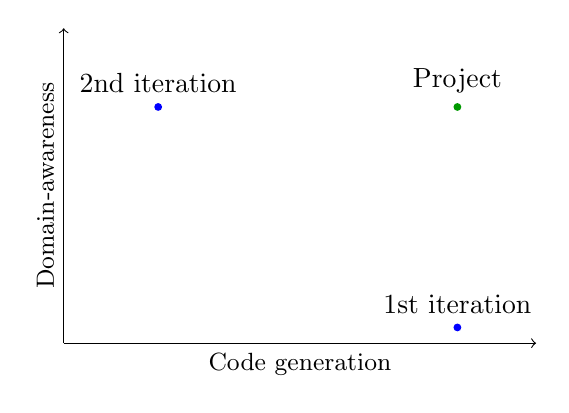
\begin{tikzpicture}
      % horizontal axis
      \draw[->] (0,0) -- (6,0) node[anchor=north,midway] {\small Code generation};

      % vertical axis
      \draw[->] (0,0) -- (0,4) node[anchor=south,rotate=90,midway] {\small Domain-awareness};

      \draw (5,0.2) node[circle,fill,inner sep=1pt, fill=blue, label=above:1st iteration] {};
      \draw (1.2,3.0) node[circle,fill,inner sep=1pt, fill=blue, label=above:2nd iteration] {};

      % Project dot
      \draw (5,3) node[circle,fill,inner sep=1pt, fill=dkgreen, label=above:Project] {}; 
    \end{tikzpicture}
    \caption{Project parameters and key points}
  \end{figure}
}

%-----------------------
% Test support tools

\section{Test support tools}
\frame {
  \begin{tikzpicture}[remember picture,overlay]
    \node[text=black, text opacity=1.0,
          font=\scriptsize] at (current page.center) {\Huge Test support tools};
  \end{tikzpicture}
}

\frame {
  \frametitle{Test support tools}
  \begin{itemize}
    \item Actor classes
    \item Interface bindings
    \item Mapping functions
  \end{itemize}
}

\frame {
  \frametitle{Test support tools - actor example} 

  \begin{figure}[!htbp]
    \centering
    \includegraphics[scale=0.60]{\imgdir support-tools-recepionist-example}
    \caption{Example composition of a receptionist actor class using a client class}
    \label{fig:support-tools-recepionist-example}
  \end{figure}
}

\frame {
  \frametitle{Structure of use cases}
  Components:
  \begin{itemize}
    \item Participating actors
    \item Ordered list of steps (scenario)
    \item Set of ordered lists of steps (extensions)
  \end{itemize}
}

%TODO if there is time.
%\frame {
%  \frametitle{Mapping function example}
%  
%  \begin{lstlisting}[style=Dart, caption=User logging in]
%  static void user_log_in(User user, 
%                          AuthenticationModule authModule) {
%   
%    expect (authModule.authenticate(user), equals(true));
%  }
%%  \end{lstlisting}
% 
%}


\frame {
  \frametitle{Representing use cases}
\begin{figure}[!htbp]
\centering
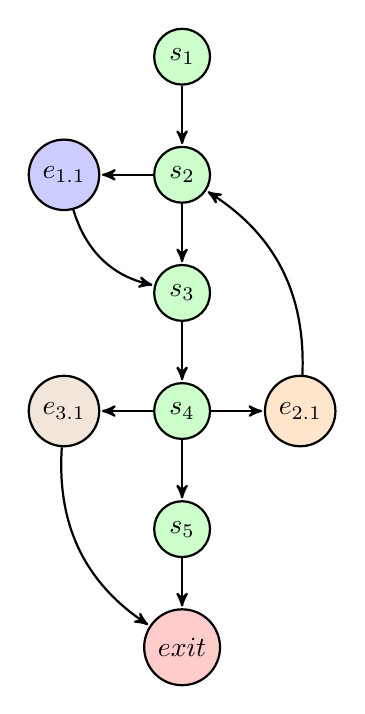
\begin{tikzpicture}[->,>=stealth',shorten >=0.6pt,auto,node distance=1.5cm,
thick,
extension1 node/.style={circle,fill=blue!20,draw,font=\sffamily\bfseries},
extension2 node/.style={circle,fill=orange!20,draw,font=\sffamily\bfseries},
extension3 node/.style={circle,fill=brown!20,draw,font=\sffamily\bfseries},
exit node/.style={circle,fill=red!20,draw,font=\sffamily\bfseries},
chosen node/.style={circle,fill=green!20,draw,font=\sffamily\bfseries}]

%Scenario
\node[chosen node] (s1) {$s_1$};
\node[chosen node] (s2) [below of=s1] {$s_2$};
\node[chosen node] (s3) [below of=s2] {$s_3$};
\node[chosen node] (s4) [below of=s3] {$s_4$};
\node[chosen node] (s5) [below of=s4] {$s_5$};
\node[exit node] (exit) [below of=s5] {$exit$};

%Extension 1
\node[extension1 node] (e1_1) [left of=s2] {$e_{1.1}$};

%Extension 2
\node[extension2 node] (e2_1) [right of=s4] {$e_{2.1}$};

%Extension 3
\node[extension3 node] (e3_1) [left of=s4] {$e_{3.1}$};

%Paths
\path[every node/.style={font=\sffamily\small}]
(s1)   edge node [] {} (s2)	
(s2)   edge node [] {} (s3)
       edge node [] {} (e1_1)
(s3)   edge node [] {} (s4)
(s4)   edge node [] {} (s5)
       edge node [] {} (e2_1)
       edge node [] {} (e3_1)
(s5)   edge node [] {} (exit)

(e1_1) edge[bend right] node [] {} (s3)
(e2_1) edge[bend right] node [] {} (s2)
(e3_1) edge[bend right] node [] {} (exit)
;
\end{tikzpicture}
\end{figure}
}

\frame {
  \frametitle{Representing use cases}

  \begin{itemize}
    \item Single linear path (of steps) for main scenario.
    \item Implicit exit point.
    \item Extensions are steps with extension point and optional return point.
    \begin{itemize}
      \item Defaults to $exit$ when none is specified.
    \end{itemize}
    \item Use case paths are collected from graph paths.
  \end{itemize}
}

\frame {
  \frametitle{Participating actors/concepts of use cases}

  \begin{itemize}
    \item Inferred from definition set
    \item Definitions are defined concepts or actors
    \item Participators are used in test generation.
  \end{itemize}
}

\frame {
  \frametitle{System state for tests}

  \begin{figure}[!htbp]
     \centering
     \includegraphics[scale=0.75]{\imgdir system-state-machine-relations}
     
     \caption{State machine of the perceived system state}
  \end{figure}
  
  \begin{block}{Example}
  The use case user log in requires a user to be present. Realized by a precondition this is another use case ("administrator creates user").\\ Initial system state will need to be cleansed on every use case run.
  
  \end{block}
}

\section{Concepts}
\frame {
  \begin{tikzpicture}[remember picture,overlay]
    \node[text=black, text opacity=1.0,
          font=\scriptsize] at (current page.center) {\Huge Concepts};
  \end{tikzpicture}
}


%The concepts

\frame {
  \frametitle{Overview}
  
  \begin{figure}[ht]
    \centering
    \subfloat[Concept 1]{
      \includegraphics[width=0.3\textwidth]{\imgdir markdown_ui_mockup}

    }\hfill
    \subfloat[Concept 2]{
      \includegraphics[width=0.3\textwidth]{\imgdir test_case_ui}

    }\hfill
    \subfloat[Concept 3]{
      \includegraphics[width=0.3\textwidth]{\imgdir customer-ui-mockup-use-cases}
    }
    \caption{The different concepts worked on in course of this thesis.}
  \end{figure}
  
  \begin{itemize}
    \item Each served as a concept -> implementation -> evaluation iteration.
    \item Refined the meta model and guided design choices.
  \end{itemize}
}

%Meta models
\frame{
  \frametitle{Meta model evolution}
  
  \begin{figure}[ht]
    \centering
    \subfloat[2\textsuperscript{nd} iteration] {
      \includegraphics[width=0.4\textwidth]{\imgdir concept2_use_case_mapping}
    
    }\hfill
    \subfloat[3\textsuperscript{rd} iteration] {
      \includegraphics[width=0.4\textwidth]{\imgdir 3rd_iteration_meta_model}
    }
    \caption{Evolution of meta model from 2\textsuperscript{nd} to 3\textsuperscript{rd} concept.}
  \end{figure}

  \begin{itemize}
    \item Value of increased complexity became questionable
    \item Simplification led realizable implementation
  \end{itemize}
}

\section{Technique}
\frame {
  \begin{tikzpicture}[remember picture,overlay]
    \node[text=black, text opacity=1.0,
          font=\scriptsize] at (current page.center) {\Huge Technique};
  \end{tikzpicture}
}


\frame {
  \frametitle{Example - walk-through}
}

\frame {
  \frametitle{Writing use cases}

  \begin{figure}[ht]
    \centering
    \includegraphics[width=0.9\textwidth]{\figdir basic-use-case}
    \caption{Example use case.}
  \end{figure}
}

\frame {
  \frametitle{Hinting use cases}

  \begin{figure}[ht]
    \centering
    \includegraphics[width=0.9\textwidth]{\figdir hinted-use-case}
    \caption{Hinted use case.}
  \end{figure}
  
  \begin{itemize}
    \item Select the text that signifies actors or concepts.
    \item Add them as definitions    
  \end{itemize}
}

\frame {
  \frametitle{Mapping - template writing}

  \begin{figure}[ht]
    \centering
    \includegraphics[width=0.9\textwidth]{\figdir example-template}
    \caption{Example template.}
  \end{figure}
  
  \begin{itemize}
    \item Create template for use case (or reuse a previous one).
    \item Realize the normalized use case steps in functions.
  \end{itemize}
}

\frame {
  \frametitle{Generating test}

  \begin{figure}[ht]
    \centering
    \includegraphics[width=0.9\textwidth]{\figdir generated-test}
    \caption{Example generated test.}
  \end{figure}

  \begin{itemize}
    \item Generate a test from a selected use case and template.
    \item Running the test may be done manually.
  \end{itemize}

}



%--------------------
% Test as requirement


%\begin{lstlisting}[style=Dart, caption=Test code for single call allocation,label={lst:test-code-single-call-allocation}]
%  static void pickupAllocatedCall(Receptionist receptionist, 
%                                  Receptionist receptionist2, 
%                                  Customer callee) {
%    String receptionNumber = '12340002';
%    Model.Call allocatedCall;
%    
%    log.info ('Customer ${callee.name} dials ${receptionNumber}');
%    callee.dial (receptionNumber);
%    log.info ('Receptionist ${receptionist.user.name} hunts call.');
%    allocatedCall = receptionist.huntNextCall();
%   
%    expect (receptionist2.pickup(call), throwsA(Forbidden));
%    log.info('Test done');
%  }
%\end{lstlisting}

\section{Wrap up}
\frame {
  \begin{tikzpicture}[remember picture,overlay]
    \node[text=black, text opacity=1.0,
          font=\scriptsize] at (current page.center) {\Huge Wrap up};
  \end{tikzpicture}
}

\frame {
  \frametitle{Evaluation - metrics}
 \begin{table}[!htbp]
\centering
\begin{tabular}{ | l | r | r | r |}
   \hline
   Project        & Total (kLoc) & Test support (kLoc) & Overhead \\ \hline
   Test framework & 8.9          & 1.1                 & 10\%     \\
   PhonIO library & 2            & 2                   & 100\%    \\
   \hline
   \hline
   Total          & 10.9         & 3.1                 & \textbf{28\%}     \\
   \hline
\end{tabular}
\caption{Test framework metrics}
\label{tab:loc-metrics}
\end{table} 

\begin{table}[!htbp]
\centering
\begin{tabular}{ | l | r | r | r |}
   \hline
   Project        & Total (commits) & Test support (commits) & Overhead \\ \hline
   Test framework & 355             & 53                     & 14.9\%   \\
   PhonIO         & 68              & 68                     & 100\%    \\
   \hline
   Total          & 10.9            & 3.1                    & \textbf{28.60\%}  \\
   \hline
   
\end{tabular}
\caption{Number of commits (as of 2\textsuperscript{nd} of July, 2015)}
\label{tab:metrics-commit-count}
\end{table}

}


\frame {
 \frametitle{Findings}
 
 \begin{itemize}
  \item Generation is very limited without strict structuring.
  \item Use case path selection method is required for high coverage.
  \item Workload increase is estimated to be \emph{at least} 28\%.
  \item Test as requirement seems more feasible, but with a different scope.
 \end{itemize} 
}
%-------------
% Presentation

\section{Presentation}
\frame {
  \begin{tikzpicture}[remember picture,overlay]
    \node[text=black, text opacity=1.0,
          font=\scriptsize] at (current page.center) {\Huge Presentation};
  \end{tikzpicture}
}

\frame {
  \frametitle{Implementation overview}
  
  \begin{figure}[!htbp]
    \centering
    \includegraphics[scale=0.5]{\imgdir layered-mvc}
    \caption{Layered model-view-control architecture with test backend}
  \end{figure}
  
  \begin{itemize}
    \item Client/server MVC architecture.
    \item Server is responsible for test generation and maintenance.
  \end{itemize}
}


\frame {
 \frametitle{State of implementation}
 \begin{itemize}
   \item Server: 
  \begin{itemize}
    \item Persistent storage of use cases, definitions and templates
    \item Generation of test from requirements
    \item Exposes REST interface for the above
  \end{itemize}
  \item Client: 
  \begin{itemize}
    \item Visualizes and manages use cases, definitions and templates
    \item Request generation of test from requirements
    \item Has incomplete \emph{visual} model for use cases
  \end{itemize}
 \end{itemize}
}

\frame {
 \frametitle{Summary}
 \begin{itemize}
   \item Gains: 
  \begin{itemize}
    \item Closer relationship between requirements and implementation
    \item More testing -- better software
    \item Mapping technique works without structuring
    \item Good fit for us -- even without generation
  \end{itemize}
  \item Losses: 
  \begin{itemize}
    \item Informal structure (instead, fixed structure for use cases)
    \item Requires \emph{ad hoc} import/export tools
    \item Time/cost increase
  \end{itemize}
 \end{itemize}
  
}

\bibliographystyle{plain}
\bibliography{../Thesis/bibliography/Bibliography.bib}

\end{document}